\documentclass[10pt]{article}
\usepackage[margin=0.55in,top=0.62in,bottom=0.6in,headsep=5pt,footskip=16pt]{geometry}
\usepackage{amsmath, amssymb}
\usepackage{xcolor}
\usepackage{booktabs}
\usepackage{tabularx}
\usepackage{array}
\usepackage{tikz}
\usepackage{needspace}
\usepackage{algpseudocode}
\usepackage{fancyhdr}

\definecolor{tgtc}{HTML}{C62828}
\definecolor{newc}{HTML}{2E7D32}
\definecolor{headc}{HTML}{1F3864}
\definecolor{barc}{HTML}{FBE3D6}

\setlength{\parindent}{0pt}
\setlength{\parskip}{2pt plus 1pt}
\newcolumntype{Y}{>{\raggedright\arraybackslash}X}
\setlength{\tabcolsep}{3.5pt}
\setlength{\aboverulesep}{0.2ex}\setlength{\belowrulesep}{0.3ex}

\pagestyle{fancy}\fancyhf{}
\fancyhead[L]{\scriptsize EECE 7205 \textbar\ Assignment 2}
\fancyhead[R]{\scriptsize MyungJin Suh}
\fancyfoot[C]{\scriptsize\thepage}
\renewcommand{\headrulewidth}{0.3pt}

\algrenewcommand\algorithmicrequire{\textbf{Input:}}
\algrenewcommand\algorithmicensure{\textbf{Output:}}
\newcommand{\Init}[1]{\item[\textbf{Initial call:}] #1}
\newcommand{\nul}[1]{NULL\,{\tiny(#1)}}
\newenvironment{algo}[2]{\par\noindent\rule{\linewidth}{0.6pt}\\[-0.1em]{\small\textbf{#1}\ \ #2}\\[-0.85em]\rule{\linewidth}{0.3pt}\footnotesize\begin{algorithmic}[1]}{\end{algorithmic}\vspace{-0.7em}\noindent\rule{\linewidth}{0.6pt}\par}

% two columns: \Lcol ... \Rcol ... \Ecol. Each row is measured; the height of a
% question's first row is saved in the .aux so the heading can be kept with it.
\makeatletter
\newsavebox\rowbox
\newcounter{qnum}
\newif\iffirstrow
\newcommand{\qrowh}[2]{\expandafter\gdef\csname qrowh@#1\endcsname{#2}}
\newcommand{\Lcol}[1][0.505]{\par\noindent\setbox\rowbox=\hbox to\linewidth\bgroup\begin{minipage}[t]{#1\linewidth}\vspace{0pt}}
\newcommand{\Rcol}[1][0.47]{\end{minipage}\hfill\begin{minipage}[t]{#1\linewidth}\vspace{0pt}}
\newcommand{\Ecol}{\end{minipage}\egroup
  \iffirstrow\immediate\write\@auxout{\string\qrowh{\theqnum}{\the\dimexpr\ht\rowbox+\dp\rowbox\relax}}\global\firstrowfalse\fi
  \noindent\usebox\rowbox\par\vspace{3pt}}
\newcommand{\qhead}[3]{\par\vspace{5pt}\stepcounter{qnum}\global\firstrowtrue
  \@ifundefined{qrowh@\theqnum}{\Needspace{12\baselineskip}}{\Needspace{\dimexpr\csname qrowh@\theqnum\endcsname+7\baselineskip\relax}}%
  \noindent\colorbox{barc}{\parbox{\dimexpr\linewidth-2\fboxsep}{\bfseries\color{headc}Question #1 (#2 points)\quad #3}}\par\vspace{1pt}}
\makeatother
\newcommand{\pt}[1]{{\bfseries\color{headc}#1}\ }
\newcommand{\fhead}[1][Count]{Line & Operation & Cost & Freq. & #1 \\ \midrule}

\tikzset{
  bn/.style={circle, draw, thick, fill=white, minimum size=4.6mm, inner sep=0pt, font=\scriptsize},
  bt/.style={every node/.style={bn}, level distance=7mm, level 1/.style={sibling distance=16mm},
             level 2/.style={sibling distance=8mm}, level 3/.style={sibling distance=6mm}, edge from parent/.style={draw, thick}},
  hl/.style={draw=newc, line width=1.3pt}, tg/.style={draw=tgtc, line width=1.3pt},
  gap/.style={draw=tgtc, dashed, thick, font=\tiny, text=tgtc},
  dl/.style={draw=none, fill=none, minimum size=0pt, inner sep=0.5pt, font=\tiny, text=tgtc}
}

\begin{document}
{\large\bfseries Assignment 2}\hfill MyungJin Suh \quad {\small EECE 7205, Fall 2026}

\vspace{2pt}
\noindent\begin{minipage}[c]{0.2\linewidth}\centering
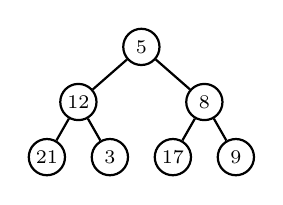
\begin{tikzpicture}[bt]
\node{5} child{node{12} child{node{21}} child{node{3}}} child{node{8} child{node{17}} child{node{9}}};
\end{tikzpicture}\\[-1pt]{\scriptsize arr $=\{5,12,8,21,3,17,9\}$, $n=7$, $h=2$}
\end{minipage}\hfill
\begin{minipage}[c]{0.78\linewidth}\footnotesize
\textbf{Counting conventions.} Every numbered line costs 1 and is counted each time it runs (a test each time it is evaluated). The \textbf{procedure} header, \textbf{else} and lines that only end a block are not counted, nor is the initial call (as in the Merge/Quick Sort handouts); a recursive call is counted once on the line that makes it. A \textbf{for} loop gives three rows: initialization, test, increment (as in the Selection Sort handout). A tree with $n$ nodes has $2n$ child pointers, $n-1$ of them edges, so $n+1$ NULL pointers; a recursive procedure called on every node and every NULL child is therefore called $1+2n = 2n+1$ times (once initially, twice by each real node).
\end{minipage}

%==================================================================
\qhead{1}{5}{Maximum depth of a binary tree}
\pt{Idea.} Depth below a node $=$ 1 $+$ the depth of its deeper subtree; an empty subtree has depth $-1$, so a leaf gets $1+\max(-1,-1)=0$. Both subtrees answer first (postorder).

\Lcol
\pt{(a) Pseudocode}
\begin{algo}{Algorithm 1}{Maximum Depth}
\Require pointer node to the root of a binary tree
\Ensure edges on the longest root-to-leaf path ($-1$ if empty)
\Init{\Call{MaxDepth}{root}}
\Procedure{MaxDepth}{node}
  \If{node $=$ NULL}
    \State \Return $-1$
  \EndIf
  \State leftDepth $\gets$ \Call{MaxDepth}{node.left}
  \State rightDepth $\gets$ \Call{MaxDepth}{node.right}
  \State \Return $1 + \max(\text{leftDepth}, \text{rightDepth})$
\EndProcedure
\end{algo}
\Rcol
\pt{(b) Worked example} {\footnotesize Real node: lines 2, 5--7; NULL: lines 2, 3.}\par
{\scriptsize
\begin{tabularx}{\linewidth}{@{}r l l Y@{}}
\toprule
\# & Call & Lines & Returns \\
\midrule
1 & 5 & 2,5--7 & $1+\max(1,1)=2$ \\
2 & 12 & 2,5--7 & $1+\max(0,0)=1$ \\
3 & 21 & 2,5--7 & $1+\max(-1,-1)=0$ \\
4 & \nul{21.L} & 2,3 & $-1$ \\
5 & \nul{21.R} & 2,3 & $-1$ \\
6 & 3 & 2,5--7 & $1+\max(-1,-1)=0$ \\
7 & \nul{3.L} & 2,3 & $-1$ \\
8 & \nul{3.R} & 2,3 & $-1$ \\
9 & 8 & 2,5--7 & $1+\max(0,0)=1$ \\
10 & 17 & 2,5--7 & $1+\max(-1,-1)=0$ \\
11 & \nul{17.L} & 2,3 & $-1$ \\
12 & \nul{17.R} & 2,3 & $-1$ \\
13 & 9 & 2,5--7 & $1+\max(-1,-1)=0$ \\
14 & \nul{9.L} & 2,3 & $-1$ \\
15 & \nul{9.R} & 2,3 & $-1$ \\
\bottomrule
\end{tabularx}}
{\footnotesize Output \textbf{2} $=$ expected. 15 calls $=2n+1$ (7 real, 8 NULL).}
\Ecol
\Lcol[0.49]
\pt{(c) Frequency count}\par
{\footnotesize\begin{tabularx}{\linewidth}{@{}c Y c c c@{}}\toprule\fhead
2 & test node $=$ NULL & 1 & $2n+1$ & 15 \\
3 & return $-1$ & 1 & $n+1$ & 8 \\
5 & left recursive call & 1 & $n$ & 7 \\
6 & right recursive call & 1 & $n$ & 7 \\
7 & return $1+\max$ & 1 & $n$ & 7 \\ \midrule
 & \textbf{Total $T(n)$} & & $\mathbf{6n+2}$ & \textbf{44} \\ \bottomrule
\end{tabularx}}
{\footnotesize Check: $6(7)+2=44$; trace: $7\times4 + 8\times2 = 44$.~\checkmark}
\Rcol[0.49]
\pt{(d) Final complexity.} $T(n)=6n+2=\Theta(n)$; \textbf{best} $=$ \textbf{worst} $=\Theta(n)$, since every node and all $n+1$ NULL pointers are visited whatever the shape. \textbf{Extra space} $\Theta(h)$ (at most $h+2$ frames): $\Theta(\log n)$ for a complete tree (4 frames here), $\Theta(n)$ worst. No input is slower in time; for space the worst input is a chain ($h=n-1$).
\Ecol
\pt{Twist (chain of 7).} The count does not change: a chain still has 7 real nodes (15 calls) and $n+1=8$ NULL pointers, so $T(7)=44$. Only the answer (6) and the stack depth (8 frames, $\Theta(n)$ space) change.

%==================================================================
\qhead{2}{5}{Sum of all nodes}
\pt{Idea.} sum $=$ root value $+$ the sums of both subtrees; an empty tree sums to 0. The queue version is level order (rule T5) with a running total.

\Lcol
\pt{(a) Pseudocode}
\begin{algo}{Algorithm 2a}{Sum (recursive)}
\Require pointer node to the root
\Ensure sum of all values (0 if empty)
\Init{\Call{Sum}{root}}
\Procedure{Sum}{node}
  \If{node $=$ NULL}
    \State \Return 0
  \EndIf
  \State leftSum $\gets$ \Call{Sum}{node.left}
  \State rightSum $\gets$ \Call{Sum}{node.right}
  \State \Return node.data $+$ leftSum $+$ rightSum
\EndProcedure
\end{algo}

\Rcol
\pt{(b) Worked example} {\footnotesize 2a: real node lines 2, 5--7; NULL lines 2, 3.}\par
{\scriptsize
\begin{tabularx}{\linewidth}{@{}r l l Y@{}}
\toprule
\# & Call & Lines & Returns \\
\midrule
1 & 5 & 2,5--7 & $5+36+34=75$ \\
2 & 12 & 2,5--7 & $12+21+3=36$ \\
3 & 21 & 2,5--7 & $21+0+0=21$ \\
4 & \nul{21.L} & 2,3 & 0 \\
5 & \nul{21.R} & 2,3 & 0 \\
6 & 3 & 2,5--7 & $3+0+0=3$ \\
7 & \nul{3.L} & 2,3 & 0 \\
8 & \nul{3.R} & 2,3 & 0 \\
9 & 8 & 2,5--7 & $8+17+9=34$ \\
10 & 17 & 2,5--7 & $17+0+0=17$ \\
11 & \nul{17.L} & 2,3 & 0 \\
12 & \nul{17.R} & 2,3 & 0 \\
13 & 9 & 2,5--7 & $9+0+0=9$ \\
14 & \nul{9.L} & 2,3 & 0 \\
15 & \nul{9.R} & 2,3 & 0 \\
\bottomrule
\end{tabularx}}
\Ecol
\Lcol
\begin{algo}{Algorithm 2b}{Sum (queue, level order)}
\Require pointer root to the root
\Ensure sum of all values (0 if empty)
\Init{\Call{SumQueue}{root}}
\Procedure{SumQueue}{root}
  \If{root $=$ NULL}
    \State \Return 0
  \EndIf
  \State total $\gets$ 0
  \State Q $\gets$ empty queue
  \State \Call{Enqueue}{Q, root}
  \While{Q is not empty}
    \State node $\gets$ \Call{Dequeue}{Q}
    \State total $\gets$ total $+$ node.data
    \If{node.left $\neq$ NULL}
      \State \Call{Enqueue}{Q, node.left}
    \EndIf
    \If{node.right $\neq$ NULL}
      \State \Call{Enqueue}{Q, node.right}
    \EndIf
  \EndWhile
  \State \Return total
\EndProcedure
\end{algo}
\Rcol
{\footnotesize 2b, one row per pass (queue front first):}\par
{\scriptsize
\begin{tabularx}{\linewidth}{@{}r Y c l l Y@{}}
\toprule
Pass & Queue before & Deq. & total & Enqueue & Queue after \\
\midrule
1 & 5 & 5 & 0+5=5 & 12, 8 & 12, 8 \\
2 & 12, 8 & 12 & 5+12=17 & 21, 3 & 8, 21, 3 \\
3 & 8, 21, 3 & 8 & 17+8=25 & 17, 9 & 21, 3, 17, 9 \\
4 & 21, 3, 17, 9 & 21 & 25+21=46 & none & 3, 17, 9 \\
5 & 3, 17, 9 & 3 & 46+3=49 & none & 17, 9 \\
6 & 17, 9 & 17 & 49+17=66 & none & 9 \\
7 & 9 & 9 & 66+9=75 & none & empty \\
\bottomrule
\end{tabularx}}
{\footnotesize Both return \textbf{75} $=$ expected; line 8 is tested an 8th time and stops.}
\Ecol
\Lcol[0.485]
\pt{(c) Frequency count} {\footnotesize 2a (same rows as Algorithm 1):}\par
{\footnotesize\begin{tabularx}{\linewidth}{@{}c Y c c c@{}}\toprule\fhead
2 & test node $=$ NULL & 1 & $2n+1$ & 15 \\
3 & return 0 & 1 & $n+1$ & 8 \\
5 & left recursive call & 1 & $n$ & 7 \\
6 & right recursive call & 1 & $n$ & 7 \\
7 & return the sum & 1 & $n$ & 7 \\ \midrule
 & \textbf{Total} & & $\mathbf{6n+2}$ & \textbf{44} \\ \bottomrule
\end{tabularx}}

\pt{(d) Final complexity.} Both $\Theta(n)$ in the \textbf{best} and \textbf{worst} case: each node is processed once whatever the shape. \textbf{Extra space:} 2a $\Theta(h)$ (stack), 2b $\Theta(w)$ (queue, $w$ = max width); both peak at 4 here. Worst input: a chain for 2a, a complete tree (last level $\approx n/2$) for 2b.
\Rcol[0.49]
{\footnotesize 2b: $n_L+n_R=n-1$ (every node but the root is enqueued once).}\par
{\footnotesize\begin{tabularx}{\linewidth}{@{}c Y c c c@{}}\toprule\fhead
2 & test root $=$ NULL & 1 & 1 & 1 \\
5 & total $\gets$ 0 & 1 & 1 & 1 \\
6 & Q $\gets$ empty queue & 1 & 1 & 1 \\
7 & Enqueue(Q, root) & 1 & 1 & 1 \\
8 & test Q not empty & 1 & $n+1$ & 8 \\
9 & node $\gets$ Dequeue(Q) & 1 & $n$ & 7 \\
10 & total $\gets$ total $+$ data & 1 & $n$ & 7 \\
11 & test left $\neq$ NULL & 1 & $n$ & 7 \\
12 & Enqueue left & 1 & $n_L$ & 3 \\
14 & test right $\neq$ NULL & 1 & $n$ & 7 \\
15 & Enqueue right & 1 & $n_R$ & 3 \\
18 & return total & 1 & 1 & 1 \\ \midrule
 & \textbf{Total} & & $\mathbf{6n+5}$ & \textbf{47} \\ \bottomrule
\end{tabularx}}
\Ecol
\pt{Twist.} Time is almost the same ($6n+2$ vs.\ $6n+5$: three set-up lines). Space goes opposite ways: a complete tree has $h=\lfloor\log_2 n\rfloor$ but $w\approx(n+1)/2$, so recursion $\Theta(\log n)$ vs.\ queue $\Theta(n)$; a chain has $h=n-1$, $w=1$, so recursion $\Theta(n)$ vs.\ queue $\Theta(1)$.

%==================================================================
\qhead{3}{5}{Count the nodes that have exactly one child}
\noindent\begin{minipage}[c]{0.74\linewidth}
\pt{Input.} INSERT(root, 4): with $n=7$, rule I6 puts 4 at index 7, parent $(7-1)/2=3$ (node 21); 7 is odd, so 4 is the \emph{left} child (I3). Now $n=8$, level order 5, 12, 8, 21, 3, 17, 9, 4.\\
\pt{Idea.} Count one-child nodes in both subtrees, then add 1 if exactly one of the node's two pointers is NULL (postorder).
\end{minipage}\hfill
\begin{minipage}[c]{0.24\linewidth}\centering
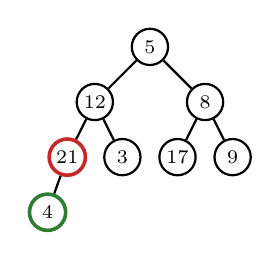
\begin{tikzpicture}[bt, level 1/.style={sibling distance=14mm}, level 2/.style={sibling distance=7mm}, level 3/.style={sibling distance=5mm}]
\node{5} child{node{12} child{node[tg]{21} child{node[hl]{4}} child[missing]} child{node{3}}} child{node{8} child{node{17}} child{node{9}}};
\end{tikzpicture}
\end{minipage}

\Lcol
\pt{(a) Pseudocode}
\begin{algo}{Algorithm 3}{Nodes with exactly one child}
\Require pointer node to the root
\Ensure number of nodes with exactly one child
\Init{\Call{OneChild}{root}}
\Procedure{OneChild}{node}
  \If{node $=$ NULL}
    \State \Return 0
  \EndIf
  \State leftCount $\gets$ \Call{OneChild}{node.left}
  \State rightCount $\gets$ \Call{OneChild}{node.right}
  \If{(node.left $=$ NULL) \textbf{xor} (node.right $=$ NULL)}
    \State \Return $1 +$ leftCount $+$ rightCount
  \EndIf
  \State \Return leftCount $+$ rightCount
\EndProcedure
\end{algo}
\Rcol
\pt{(b) Worked example} {\footnotesize On the 8-node tree.}\par
{\scriptsize
\begin{tabularx}{\linewidth}{@{}r l l Y@{}}
\toprule
\# & Call & Lines & Returns \\
\midrule
1 & 5 & 2,5--7,10 & $1+0=1$ \\
2 & 12 & 2,5--7,10 & $1+0=1$ \\
3 & 21 & 2,5--8 & $1+0+0=1$ \\
4 & 4 & 2,5--7,10 & $0+0=0$ \\
5 & \nul{4.L} & 2,3 & 0 \\
6 & \nul{4.R} & 2,3 & 0 \\
7 & \nul{21.R} & 2,3 & 0 \\
8 & 3 & 2,5--7,10 & $0+0=0$ \\
9 & \nul{3.L} & 2,3 & 0 \\
10 & \nul{3.R} & 2,3 & 0 \\
11 & 8 & 2,5--7,10 & $0+0=0$ \\
12 & 17 & 2,5--7,10 & $0+0=0$ \\
13 & \nul{17.L} & 2,3 & 0 \\
14 & \nul{17.R} & 2,3 & 0 \\
15 & 9 & 2,5--7,10 & $0+0=0$ \\
16 & \nul{9.L} & 2,3 & 0 \\
17 & \nul{9.R} & 2,3 & 0 \\
\bottomrule
\end{tabularx}}
{\footnotesize Output \textbf{1} (node 21) $=$ expected; 17 calls $=2n+1$.}
\Ecol
\Lcol[0.49]
\pt{(c) Frequency count} {\footnotesize $k$ = one-child nodes ($k=1$); each real node returns via line 8 or 10, so $k$ cancels.}\par
{\footnotesize\begin{tabularx}{\linewidth}{@{}c Y c c c@{}}\toprule\fhead[Count ($n{=}8$)]
2 & test node $=$ NULL & 1 & $2n+1$ & 17 \\
3 & return 0 & 1 & $n+1$ & 9 \\
5 & left recursive call & 1 & $n$ & 8 \\
6 & right recursive call & 1 & $n$ & 8 \\
7 & test exactly one child & 1 & $n$ & 8 \\
8 & return $1+\dots$ & 1 & $k$ & 1 \\
10 & return $\dots$ & 1 & $n-k$ & 7 \\ \midrule
 & \textbf{Total} & & $\mathbf{7n+2}$ & \textbf{58} \\ \bottomrule
\end{tabularx}}
\Rcol[0.49]
\pt{(d) Final complexity.} $T(n)=7n+2=\Theta(n)$, \textbf{best} $=$ \textbf{worst} $=\Theta(n)$: every node must be inspected. \textbf{Extra space} $\Theta(h)$; a chain is the worst input for space.
\Ecol
\pt{Twist.} In an array-built tree node $i$ has a left child iff $2i+1\le n-1$ and a right child iff $2i+2\le n-1$. Exactly one child iff $2i+1 \le n-1 < 2i+2$, i.e.\ $n = 2i+2$. For even $n\ge2$ the only solution is $i=n/2-1$ (one node); for odd $n$ there is none because $2i+2$ is even. Here $n=8$ gives $i=3$, node 21; before the insertion $n=7$ and the count was 0.

%==================================================================
\qhead{4}{5}{Are two trees identical?}
\noindent\begin{minipage}[c]{0.74\linewidth}
\pt{Idea.} Walk both trees in preorder in lockstep: two NULLs match; one NULL means the shapes differ; different values mean the trees differ; otherwise compare the left pair, and the right pair only if the left matched. The first difference ends the walk.
\end{minipage}\hfill
\begin{minipage}[c]{0.24\linewidth}\centering
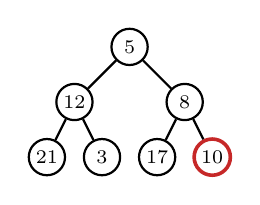
\begin{tikzpicture}[bt, level 1/.style={sibling distance=14mm}, level 2/.style={sibling distance=7mm}]
\node{5} child{node{12} child{node{21}} child{node{3}}} child{node{8} child{node{17}} child{node[tg]{10}}};
\end{tikzpicture}\\[-1pt]{\scriptsize tree C}
\end{minipage}

\Lcol
\pt{(a) Pseudocode}
\begin{algo}{Algorithm 4}{Identical trees}
\Require roots a, b of two binary trees
\Ensure true iff same shape and same values
\Init{\Call{Identical}{rootA, rootB}}
\Procedure{Identical}{a, b}
  \If{a $=$ NULL \textbf{and} b $=$ NULL}
    \State \Return true
  \EndIf
  \If{a $=$ NULL \textbf{or} b $=$ NULL}
    \State \Return false
  \EndIf
  \If{a.data $\neq$ b.data}
    \State \Return false
  \EndIf
  \If{\Call{Identical}{a.left, b.left} $=$ false}
    \State \Return false
  \EndIf
  \State \Return \Call{Identical}{a.right, b.right}
\EndProcedure
\end{algo}
\Rcol
\pt{(b) Worked example} {\footnotesize IDENTICAL(A, B) $=$ \textbf{true}:}\par
{\scriptsize
\begin{tabularx}{\linewidth}{@{}r l l Y@{}}
\toprule
\# & Pair & Lines & Returns \\
\midrule
1 & (5, 5) & 2,5,8,11,14 & true \\
2 & (12, 12) & 2,5,8,11,14 & true \\
3 & (21, 21) & 2,5,8,11,14 & true \\
4 & (N, N) {\tiny(21.L)} & 2,3 & true \\
5 & (N, N) {\tiny(21.R)} & 2,3 & true \\
6 & (3, 3) & 2,5,8,11,14 & true \\
7 & (N, N) {\tiny(3.L)} & 2,3 & true \\
8 & (N, N) {\tiny(3.R)} & 2,3 & true \\
9 & (8, 8) & 2,5,8,11,14 & true \\
10 & (17, 17) & 2,5,8,11,14 & true \\
11 & (N, N) {\tiny(17.L)} & 2,3 & true \\
12 & (N, N) {\tiny(17.R)} & 2,3 & true \\
13 & (9, 9) & 2,5,8,11,14 & true \\
14 & (N, N) {\tiny(9.L)} & 2,3 & true \\
15 & (N, N) {\tiny(9.R)} & 2,3 & true \\
\bottomrule
\end{tabularx}}
\Ecol
\Lcol
{\footnotesize IDENTICAL(A, C) $=$ \textbf{false} (same first 12 calls; call 13 finds $9\ne10$ and the false is passed up through line 14):}\par
{\scriptsize
\begin{tabularx}{\linewidth}{@{}r l l Y@{}}
\toprule
\# & Pair & Lines & Returns \\
\midrule
1 & (5, 5) & 2,5,8,11,14 & false \\
2 & (12, 12) & 2,5,8,11,14 & true \\
3 & (21, 21) & 2,5,8,11,14 & true \\
4 & (N, N) {\tiny(21.L)} & 2,3 & true \\
5 & (N, N) {\tiny(21.R)} & 2,3 & true \\
6 & (3, 3) & 2,5,8,11,14 & true \\
7 & (N, N) {\tiny(3.L)} & 2,3 & true \\
8 & (N, N) {\tiny(3.R)} & 2,3 & true \\
9 & (8, 8) & 2,5,8,11,14 & false \\
10 & (17, 17) & 2,5,8,11,14 & true \\
11 & (N, N) {\tiny(17.L)} & 2,3 & true \\
12 & (N, N) {\tiny(17.R)} & 2,3 & true \\
13 & (9, 10) & 2,5,8,9 & false ($9\ne10$) \\
\bottomrule
\end{tabularx}}
{\footnotesize Both results match the expected output.}
\Rcol
\pt{(c) Frequency count} {\footnotesize worst case $=$ identical trees.}\par
{\footnotesize\begin{tabularx}{\linewidth}{@{}c Y c c c c@{}}\toprule
Line & Operation & Cost & Freq. & (A,B) & (A,C) \\ \midrule
2 & test both NULL & 1 & $2n+1$ & 15 & 13 \\
3 & return true & 1 & $n+1$ & 8 & 6 \\
5 & test one NULL & 1 & $n$ & 7 & 7 \\
6 & return false & 1 & 0 & 0 & 0 \\
8 & test data differ & 1 & $n$ & 7 & 7 \\
9 & return false & 1 & 0 & 0 & 1 \\
11 & test left pair & 1 & $n$ & 7 & 6 \\
12 & return false & 1 & 0 & 0 & 0 \\
14 & return right pair & 1 & $n$ & 7 & 6 \\ \midrule
 & \textbf{Total} & & $\mathbf{7n+2}$ & \textbf{51} & \textbf{46} \\ \bottomrule
\end{tabularx}}
\Ecol
\pt{(d) Final complexity.} \textbf{Worst} $\Theta(n)$ ($7n+2$): identical trees, or trees that differ only at the last pair in preorder, since every pair must be compared. \textbf{Best} $\Theta(1)$: the roots differ (lines 2, 5, 8, 9). \textbf{Extra space} $\Theta(h)$.
\pt{Twist.} IDENTICAL(A, C) first finds a difference at call 13, the pair (9, 10) under 8: the \emph{last} node in preorder (5, 12, 21, 3, 8, 17, 9), so it costs 46 of the 51 lines of a full match (it skips the two NULL pairs under 9 and lines 11, 14 there, but runs line 9). For two trees of $n$ nodes: best $\Theta(1)$ (roots differ), worst $\Theta(n)$ (identical).

%==================================================================
\qhead{5}{5}{Minimum value in a binary tree}
\pt{Idea.} The tree is unordered, so take the min of the node's value and both subtree minima; NULL returns $+\infty$, which never wins.

\Lcol
\pt{(a) Pseudocode}
\begin{algo}{Algorithm 5}{Minimum value}
\Require pointer node to the root
\Ensure smallest value ($+\infty$ if empty)
\Init{\Call{MinValue}{root}}
\Procedure{MinValue}{node}
  \If{node $=$ NULL}
    \State \Return $+\infty$
  \EndIf
  \State leftMin $\gets$ \Call{MinValue}{node.left}
  \State rightMin $\gets$ \Call{MinValue}{node.right}
  \State \Return $\min(\text{node.data}, \text{leftMin}, \text{rightMin})$
\EndProcedure
\end{algo}
\Rcol
\pt{(b) Worked example}\par
{\scriptsize
\begin{tabularx}{\linewidth}{@{}r l l Y@{}}
\toprule
\# & Call & Lines & Returns \\
\midrule
1 & 5 & 2,5--7 & $\min(5,3,8)=3$ \\
2 & 12 & 2,5--7 & $\min(12,21,3)=3$ \\
3 & 21 & 2,5--7 & $\min(21,\infty,\infty)=21$ \\
4 & \nul{21.L} & 2,3 & $+\infty$ \\
5 & \nul{21.R} & 2,3 & $+\infty$ \\
6 & 3 & 2,5--7 & $\min(3,\infty,\infty)=3$ \\
7 & \nul{3.L} & 2,3 & $+\infty$ \\
8 & \nul{3.R} & 2,3 & $+\infty$ \\
9 & 8 & 2,5--7 & $\min(8,17,9)=8$ \\
10 & 17 & 2,5--7 & $\min(17,\infty,\infty)=17$ \\
11 & \nul{17.L} & 2,3 & $+\infty$ \\
12 & \nul{17.R} & 2,3 & $+\infty$ \\
13 & 9 & 2,5--7 & $\min(9,\infty,\infty)=9$ \\
14 & \nul{9.L} & 2,3 & $+\infty$ \\
15 & \nul{9.R} & 2,3 & $+\infty$ \\
\bottomrule
\end{tabularx}}
{\footnotesize Output \textbf{3} $=$ expected.}
\Ecol
\Lcol[0.49]
\pt{(c) Frequency count}\par
{\footnotesize\begin{tabularx}{\linewidth}{@{}c Y c c c@{}}\toprule\fhead
2 & test node $=$ NULL & 1 & $2n+1$ & 15 \\
3 & return $+\infty$ & 1 & $n+1$ & 8 \\
5 & left recursive call & 1 & $n$ & 7 \\
6 & right recursive call & 1 & $n$ & 7 \\
7 & return the min & 1 & $n$ & 7 \\ \midrule
 & \textbf{Total} & & $\mathbf{6n+2}$ & \textbf{44} \\ \bottomrule
\end{tabularx}}
\Rcol[0.49]
\pt{(d) Final complexity.} $\Theta(n)$ \textbf{best} and \textbf{worst}: without order any unvisited node could be smaller. \textbf{Extra space} $\Theta(h)$, worst for a chain.
\Ecol
\Lcol[0.37]
\begin{algo}{Algorithm 5b}{Minimum in a BST}
\Require root of a non-empty BST
\Ensure smallest value
\Init{\Call{BSTMin}{root}}
\Procedure{BSTMin}{root}
  \State node $\gets$ root
  \While{node.left $\neq$ NULL}
    \State node $\gets$ node.left
  \EndWhile
  \State \Return node.data
\EndProcedure
\end{algo}
\Rcol[0.6]
\pt{Twist (BST).} In a BST the minimum is the \emph{leftmost} node: follow left pointers, no recursion. With $d$ the depth of the leftmost node, line 2 runs once, line 3 $d+1$ times, line 4 $d$ times, line 6 once: $T=2d+3$. On S $=\{9,5,17,3,8,12,21\}$ (Q14): $9\to5\to3$, $d=2$, $T=7$, returns 3. Cost becomes $\Theta(h)$: best $\Theta(1)$ (no left child at the root), $\Theta(\log n)$ balanced, worst $\Theta(n)$ (left chain); extra space $\Theta(1)$.
\Ecol

%==================================================================
\qhead{6}{7}{Invert (mirror) a binary tree}
\noindent\begin{minipage}[c]{0.6\linewidth}
\pt{Idea.} Invert both subtrees, then attach the inverted right subtree on the left and the inverted left subtree on the right (postorder). Each node's two pointers are swapped exactly once; NULL children stay NULL.
\end{minipage}\hfill
\begin{minipage}[c]{0.38\linewidth}\centering
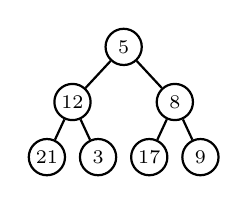
\begin{tikzpicture}[bt, level 1/.style={sibling distance=13mm}, level 2/.style={sibling distance=6.5mm}]
\node{5} child{node{12} child{node{21}} child{node{3}}} child{node{8} child{node{17}} child{node{9}}};
\end{tikzpicture}\ \raisebox{5mm}{$\Rightarrow$}\
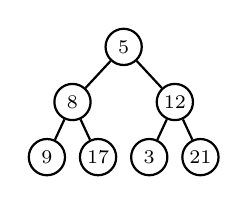
\begin{tikzpicture}[bt, level 1/.style={sibling distance=13mm}, level 2/.style={sibling distance=6.5mm}]
\node{5} child{node{8} child{node{9}} child{node{17}}} child{node{12} child{node{3}} child{node{21}}};
\end{tikzpicture}
\end{minipage}

\Lcol
\pt{(a) Pseudocode}
\begin{algo}{Algorithm 6}{Invert a binary tree}
\Require pointer node to the root
\Ensure root of the mirrored tree (in place)
\Init{root $\gets$ \Call{Invert}{root}}
\Procedure{Invert}{node}
  \If{node $=$ NULL}
    \State \Return NULL
  \EndIf
  \State leftInv $\gets$ \Call{Invert}{node.left}
  \State rightInv $\gets$ \Call{Invert}{node.right}
  \State node.left $\gets$ rightInv
  \State node.right $\gets$ leftInv
  \State \Return node
\EndProcedure
\end{algo}
\Rcol
\pt{(b) Worked example} {\footnotesize Swaps happen on the way back up.}\par
{\scriptsize
\begin{tabularx}{\linewidth}{@{}r l l Y l@{}}
\toprule
\# & Call & Lines & Lines 7--8 set & Ret. \\
\midrule
1 & 5 & 2,5--9 & L$\gets$8, R$\gets$12 & 5 \\
2 & 12 & 2,5--9 & L$\gets$3, R$\gets$21 & 12 \\
3 & 21 & 2,5--9 & L$\gets$N, R$\gets$N & 21 \\
4 & \nul{21.L} & 2,3 & -- & NULL \\
5 & \nul{21.R} & 2,3 & -- & NULL \\
6 & 3 & 2,5--9 & L$\gets$N, R$\gets$N & 3 \\
7 & \nul{3.L} & 2,3 & -- & NULL \\
8 & \nul{3.R} & 2,3 & -- & NULL \\
9 & 8 & 2,5--9 & L$\gets$9, R$\gets$17 & 8 \\
10 & 17 & 2,5--9 & L$\gets$N, R$\gets$N & 17 \\
11 & \nul{17.L} & 2,3 & -- & NULL \\
12 & \nul{17.R} & 2,3 & -- & NULL \\
13 & 9 & 2,5--9 & L$\gets$N, R$\gets$N & 9 \\
14 & \nul{9.L} & 2,3 & -- & NULL \\
15 & \nul{9.R} & 2,3 & -- & NULL \\
\bottomrule
\end{tabularx}}
{\footnotesize Level order after: \textbf{5, 8, 12, 9, 17, 3, 21} $=$ expected.}
\Ecol
\Lcol[0.49]
\pt{(c) Frequency count}\par
{\footnotesize\begin{tabularx}{\linewidth}{@{}c Y c c c@{}}\toprule\fhead
2 & test node $=$ NULL & 1 & $2n+1$ & 15 \\
3 & return NULL & 1 & $n+1$ & 8 \\
5 & left recursive call & 1 & $n$ & 7 \\
6 & right recursive call & 1 & $n$ & 7 \\
7 & node.left $\gets$ rightInv & 1 & $n$ & 7 \\
8 & node.right $\gets$ leftInv & 1 & $n$ & 7 \\
9 & return node & 1 & $n$ & 7 \\ \midrule
 & \textbf{Total} & & $\mathbf{8n+2}$ & \textbf{58} \\ \bottomrule
\end{tabularx}}
\Rcol[0.49]
\pt{(d) Final complexity.} $T(n)=8n+2=\Theta(n)$, \textbf{best} $=$ \textbf{worst}: every node must be rewired. \textbf{Extra space} $\Theta(h)$ (worst: chain); the inversion is in place.
\Ecol
\pt{Twist.} Inorder before: 21 12 3 5 17 8 9; after: \textbf{9 8 17 5 3 12 21}, exactly the reverse. Mirroring swaps L and R at every node, so inorder (L N R) of the mirror visits the original in R N L order (reverse inorder). By induction, with $L$, $R$ the subtrees of the root $N$: $\text{in}(\text{mir}(T)) = \text{in}(\text{mir}(R))\,N\,\text{in}(\text{mir}(L)) = \text{rev}(\text{in}(R))\,N\,\text{rev}(\text{in}(L)) = \text{rev}(\text{in}(T))$.

%==================================================================
\qhead{7}{7}{Print each level on its own line, and the right side view}
\pt{Idea.} Level order (T5), but each pass first reads size $\gets$ SIZE(Q): the queue then holds exactly one level, which the inner loop prints while enqueuing the next. The node with $i=$ size is the rightmost of its level.

\Lcol
\pt{(a) Pseudocode}
\begin{algo}{Algorithm 7}{Levels and right side view}
\Require pointer root to the root
\Ensure each level on its own line; returns the right side view
\Init{view $\gets$ \Call{LevelsAndView}{root}}
\Procedure{LevelsAndView}{root}
  \If{root $=$ NULL}
    \State \Return empty list
  \EndIf
  \State view $\gets$ empty list
  \State Q $\gets$ empty queue
  \State \Call{Enqueue}{Q, root}
  \While{Q is not empty}
    \State size $\gets$ \Call{Size}{Q}
    \For{$i \gets 1$ \textbf{to} size}
      \State node $\gets$ \Call{Dequeue}{Q}
      \State \textbf{print} node.data
      \If{node.left $\neq$ NULL}
        \State \Call{Enqueue}{Q, node.left}
      \EndIf
      \If{node.right $\neq$ NULL}
        \State \Call{Enqueue}{Q, node.right}
      \EndIf
      \If{$i =$ size}
        \State \Call{Append}{view, node.data}
      \EndIf
    \EndFor
    \State \textbf{print} newline
  \EndWhile
  \State \Return view
\EndProcedure
\end{algo}
\Rcol
\pt{(b) Worked example} {\footnotesize One row per pass (level).}\par
{\scriptsize
\begin{tabularx}{\linewidth}{@{}c Y c l c Y l@{}}
\toprule
Level & Queue before & size & Line printed & $i=$size & Queue after & view \\
\midrule
1 & 5 & 1 & 5 & 5 & 12, 8 & 5 \\
2 & 12, 8 & 2 & 12 8 & 8 & 21, 3, 17, 9 & 5, 8 \\
3 & 21, 3, 17, 9 & 4 & 21 3 17 9 & 9 & empty & 5, 8, 9 \\
\bottomrule
\end{tabularx}}
{\footnotesize Levels \textbf{[5], [12, 8], [21, 3, 17, 9]}; view \textbf{5, 8, 9} $=$ expected.}\par\vspace{3pt}
\pt{(c) Frequency count} {\footnotesize $L=h+1=3$ levels; $n_L+n_R=n-1$.}\par
{\footnotesize\begin{tabularx}{\linewidth}{@{}c Y c c c@{}}\toprule\fhead
2 & test root $=$ NULL & 1 & 1 & 1 \\
5 & view $\gets$ empty & 1 & 1 & 1 \\
6 & Q $\gets$ empty & 1 & 1 & 1 \\
7 & Enqueue(root) & 1 & 1 & 1 \\
8 & test Q not empty & 1 & $L+1$ & 4 \\
9 & size $\gets$ Size(Q) & 1 & $L$ & 3 \\
10 & for: init / test / incr. & 1 & $L$ / $n{+}L$ / $n$ & 3/10/7 \\
11 & Dequeue & 1 & $n$ & 7 \\
12 & print node.data & 1 & $n$ & 7 \\
13 & test left & 1 & $n$ & 7 \\
14 & Enqueue left & 1 & $n_L$ & 3 \\
16 & test right & 1 & $n$ & 7 \\
17 & Enqueue right & 1 & $n_R$ & 3 \\
19 & test $i=$ size & 1 & $n$ & 7 \\
20 & Append to view & 1 & $L$ & 3 \\
23 & print newline & 1 & $L$ & 3 \\
25 & return view & 1 & 1 & 1 \\ \midrule
 & \textbf{Total} & & $\mathbf{8n{+}6L{+}5}$ & \textbf{79} \\ \bottomrule
\end{tabularx}}
{\footnotesize $=8n+6h+11$; check $56+18+5=79$.~\checkmark}
\Ecol
\pt{Twist (where the terms come from).} $8n$ is the per-node work: lines 11, 12, 13, 16, 19, the inner test and increment, and the $n-1$ enqueues. $6L=6(h+1)$ is the per-level work: outer test, size, inner-loop init, its final failed test, Append to view, newline. The constant 5 is the set-up and return.
\pt{(d) Final complexity.} With $1\le L\le n$: $8n+6\lfloor\log_2 n\rfloor+11$ (complete tree) $\le T(n) \le 14n+5$ (chain, one node per level, so per-level work is paid $n$ times). \textbf{Best} $=$ \textbf{worst} $=\Theta(n)$. \textbf{Extra space} $\Theta(w)$ queue $+\ \Theta(h)$ view, $\Theta(n)$ worst.

%==================================================================
\qhead{8}{7}{Zigzag (spiral) level order traversal}
\pt{Idea.} A stack reverses what is pushed on it. S1 holds an even level (popped left to right); its nodes push children \emph{left then right} onto S2, so S2 pops right to left. S2's nodes push \emph{right then left} onto S1, so the next level pops left to right again.

\Lcol
\pt{(a) Pseudocode}
\begin{algo}{Algorithm 8a}{Zigzag with two stacks}
\Require pointer root to the root
\Ensure prints levels alternately L$\to$R and R$\to$L
\Init{\Call{ZigzagStacks}{root}}
\Procedure{ZigzagStacks}{root}
  \If{root $=$ NULL}
    \State \Return
  \EndIf
  \State S1 $\gets$ empty stack \Comment{even levels}
  \State S2 $\gets$ empty stack \Comment{odd levels}
  \State \Call{Push}{S1, root}
  \While{S1 is not empty}
    \While{S1 is not empty}
      \State node $\gets$ \Call{Pop}{S1}
      \State \textbf{print} node.data
      \If{node.left $\neq$ NULL}
        \State \Call{Push}{S2, node.left}
      \EndIf
      \If{node.right $\neq$ NULL}
        \State \Call{Push}{S2, node.right}
      \EndIf
    \EndWhile
    \While{S2 is not empty}
      \State node $\gets$ \Call{Pop}{S2}
      \State \textbf{print} node.data
      \If{node.right $\neq$ NULL}
        \State \Call{Push}{S1, node.right}
      \EndIf
      \If{node.left $\neq$ NULL}
        \State \Call{Push}{S1, node.left}
      \EndIf
    \EndWhile
  \EndWhile
\EndProcedure
\end{algo}
\Rcol
\pt{(b) Worked example} {\footnotesize One row per pop; stacks bottom to top.}\par
{\scriptsize
\begin{tabularx}{\linewidth}{@{}r c c l l l Y@{}}
\toprule
Pop & From & Node & Push & S1 after & S2 after & Output \\
\midrule
1 & S1 & 5 & S2$\gets$12, 8 & empty & 12, 8 & 5 \\
2 & S2 & 8 & S1$\gets$9, 17 & 9, 17 & 12 & 5 8 \\
3 & S2 & 12 & S1$\gets$3, 21 & 9, 17, 3, 21 & empty & 5 8 12 \\
4 & S1 & 21 & S2$\gets$none & 9, 17, 3 & empty & 5 8 12 21 \\
5 & S1 & 3 & S2$\gets$none & 9, 17 & empty & 5 8 12 21 3 \\
6 & S1 & 17 & S2$\gets$none & 9 & empty & 5 8 12 21 3 17 \\
7 & S1 & 9 & S2$\gets$none & empty & empty & 5 8 12 21 3 17 9 \\
\bottomrule
\end{tabularx}}
{\footnotesize Output \textbf{5, 8, 12, 21, 3, 17, 9} $=$ expected.}\par\vspace{3pt}
\pt{(c) Frequency count} {\footnotesize $E=\lceil L/2\rceil$ even levels $=$ outer passes ($E=2$); $n_e,n_o$ nodes on even/odd levels ($5, 2$); the four pushes total $n-1$.}\par
{\footnotesize\begin{tabularx}{\linewidth}{@{}c Y c c c@{}}\toprule\fhead
2 & test root $=$ NULL & 1 & 1 & 1 \\
5 & S1 $\gets$ empty & 1 & 1 & 1 \\
6 & S2 $\gets$ empty & 1 & 1 & 1 \\
7 & Push(S1, root) & 1 & 1 & 1 \\
8 & outer test & 1 & $E+1$ & 3 \\
9 & S1 loop test & 1 & $n_e+E$ & 7 \\
10 & Pop(S1) & 1 & $n_e$ & 5 \\
11 & print & 1 & $n_e$ & 5 \\
12 & test left & 1 & $n_e$ & 5 \\
13 & Push left on S2 & 1 & $\ell_e$ & 1 \\
15 & test right & 1 & $n_e$ & 5 \\
16 & Push right on S2 & 1 & $r_e$ & 1 \\
19 & S2 loop test & 1 & $n_o+E$ & 4 \\
20 & Pop(S2) & 1 & $n_o$ & 2 \\
21 & print & 1 & $n_o$ & 2 \\
22 & test right & 1 & $n_o$ & 2 \\
23 & Push right on S1 & 1 & $r_o$ & 2 \\
25 & test left & 1 & $n_o$ & 2 \\
26 & Push left on S1 & 1 & $\ell_o$ & 2 \\ \midrule
 & \textbf{Total} & & $\mathbf{6n{+}3E{+}4}$ & \textbf{52} \\ \bottomrule
\end{tabularx}}
{\footnotesize $\ell_e{+}r_e{+}r_o{+}\ell_o=n-1$. Check $42+6+4=52$.~\checkmark}
\Ecol
\pt{(d) Final complexity.} $E\le n$, so $T(n)$ runs from about $6n+1.5\log_2 n$ (complete) to $7.5n$ (chain, worst count: every level adds outer-loop overhead). \textbf{Best} $=$ \textbf{worst} $=\Theta(n)$. \textbf{Extra space} $\Theta(w)$: the stacks hold at most two levels.

\Lcol[0.47]
\begin{algo}{Algorithm 8b}{Zigzag with a queue and reversal}
\Require pointer root to the root
\Ensure same output as Algorithm 8a
\Init{\Call{ZigzagQueue}{root}}
\Procedure{ZigzagQueue}{root}
  \If{root $=$ NULL}
    \State \Return
  \EndIf
  \State Q $\gets$ empty queue
  \State \Call{Enqueue}{Q, root}
  \State leftToRight $\gets$ true
  \While{Q is not empty}
    \State size $\gets$ \Call{Size}{Q}
    \State level $\gets$ empty list
    \For{$i \gets 1$ \textbf{to} size}
      \State node $\gets$ \Call{Dequeue}{Q}
      \State \Call{Append}{level, node.data}
      \If{node.left $\neq$ NULL}
        \State \Call{Enqueue}{Q, node.left}
      \EndIf
      \If{node.right $\neq$ NULL}
        \State \Call{Enqueue}{Q, node.right}
      \EndIf
    \EndFor
    \If{leftToRight $=$ false}
      \State lo $\gets 0$;\ hi $\gets$ size $-1$
      \While{lo $<$ hi}
        \State \Call{Swap}{level[lo], level[hi]}
        \State lo $\gets$ lo$+1$;\ hi $\gets$ hi$-1$
      \EndWhile
    \EndIf
    \For{$j \gets 0$ \textbf{to} size $-1$}
      \State \textbf{print} level[$j$]
    \EndFor
    \State leftToRight $\gets$ \textbf{not} leftToRight
  \EndWhile
\EndProcedure
\end{algo}
\Rcol[0.505]
\pt{Twist: queue plus reversal.} One row per level:\par
{\scriptsize
\begin{tabularx}{\linewidth}{@{}c Y c l c l Y@{}}
\toprule
Lvl & Queue before & Dir. & level & Swaps & Printed & Queue after \\
\midrule
1 & 5 & L$\to$R & 5 & 0 & 5 & 12, 8 \\
2 & 12, 8 & R$\to$L & 12 8 & 1 & 8 12 & 21, 3, 17, 9 \\
3 & 21, 3, 17, 9 & L$\to$R & 21 3 17 9 & 0 & 21 3 17 9 & empty \\
\bottomrule
\end{tabularx}}
{\footnotesize With $O$ odd levels and $P$ swaps ($\lfloor\text{size}/2\rfloor$ per odd level): lines 2, 5, 6, 7 run once; line 8 $L+1$ times; lines 9, 10, 21, 31 and both for-inits $L$ times; each for-test $n+L$ times; lines 12, 13, 14, 17, 29 and both increments $n$ times; enqueues $n-1$; line 22 $O$; line 23 $P+O$; lines 24, 25 $P$ each. Total}
\[T_{8b}(n)=10n+9L+2O+3P+4,\]\[T_{8b}(7)=70+27+2+3+4=106.\]
\textbf{The two stacks do less work} (52 vs.\ 106). They handle each node once and get the zigzag order for free; the queue version handles each node twice (into the list, then printed), spends 9 lines of bookkeeping per level, and 3 lines per swap (up to $n/2$ swaps). Both are $\Theta(n)$ time, $\Theta(w)$ space.
\Ecol

%==================================================================
\qhead{9}{7}{Is the tree complete?}
\noindent\begin{minipage}[c]{0.74\linewidth}
\pt{Idea.} Level order that enqueues \emph{both} children, NULL or not. In a complete tree all real nodes precede all NULLs in level order (C6), so after the first NULL is dequeued, any real node is a gap: return false.
\end{minipage}\hfill
\begin{minipage}[c]{0.24\linewidth}\centering
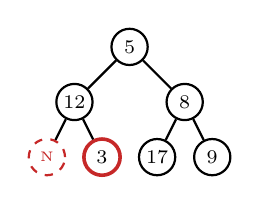
\begin{tikzpicture}[bt, level 1/.style={sibling distance=14mm}, level 2/.style={sibling distance=7mm}]
\node{5} child{node{12} child{node[gap]{N}} child{node[tg]{3}}} child{node{8} child{node{17}} child{node{9}}};
\end{tikzpicture}\\[-1pt]{\scriptsize tree Q}
\end{minipage}

\Lcol[0.45]
\pt{(a) Pseudocode}
\begin{algo}{Algorithm 9}{Complete tree check}
\Require pointer root to the root
\Ensure true iff the tree is complete
\Init{\Call{Complete}{root}}
\Procedure{Complete}{root}
  \If{root $=$ NULL}
    \State \Return true
  \EndIf
  \State Q $\gets$ empty queue
  \State \Call{Enqueue}{Q, root}
  \State seenNull $\gets$ false
  \While{Q is not empty}
    \State node $\gets$ \Call{Dequeue}{Q}
    \If{node $=$ NULL}
      \State seenNull $\gets$ true
    \Else
      \If{seenNull $=$ true}
        \State \Return false \Comment{gap}
      \EndIf
      \State \Call{Enqueue}{Q, node.left}
      \State \Call{Enqueue}{Q, node.right}
    \EndIf
  \EndWhile
  \State \Return true
\EndProcedure
\end{algo}
\Rcol[0.53]
\pt{(b) Worked example} {\footnotesize One row per pass; N$\times k$ $=$ $k$ NULLs. Tree P:}\par
{\scriptsize
\begin{tabularx}{\linewidth}{@{}r Y c l c Y@{}}
\toprule
Pass & Queue before & Deq. & Action & seen & Queue after \\
\midrule
1 & 5 & 5 & enq 12, 8 & false & 12, 8 \\
2 & 12, 8 & 12 & enq 21, 3 & false & 8, 21, 3 \\
3 & 8, 21, 3 & 8 & enq 17, 9 & false & 21, 3, 17, 9 \\
4 & 21, 3, 17, 9 & 21 & enq N, N & false & 3, 17, 9, N, N \\
5 & 3, 17, 9, N, N & 3 & enq N, N & false & 17, 9, N$\times$4 \\
6 & 17, 9, N$\times$4 & 17 & enq N, N & false & 9, N$\times$6 \\
7 & 9, N$\times$6 & 9 & enq N, N & false & N$\times$8 \\
8 & N$\times$8 & N & seenNull $\gets$ true & true & N$\times$7 \\
9 & N$\times$7 & N & seenNull $\gets$ true & true & N$\times$6 \\
10 & N$\times$6 & N & seenNull $\gets$ true & true & N$\times$5 \\
11 & N$\times$5 & N & seenNull $\gets$ true & true & N$\times$4 \\
12 & N$\times$4 & N & seenNull $\gets$ true & true & N$\times$3 \\
13 & N$\times$3 & N & seenNull $\gets$ true & true & N, N \\
14 & N, N & N & seenNull $\gets$ true & true & N \\
15 & N & N & seenNull $\gets$ true & true & empty \\
\bottomrule
\end{tabularx}}
{\footnotesize 16th test of line 8 finds the queue empty: COMPLETE(P) $=$ \textbf{true}. Tree Q $=\{5,12,8,\text{NULL},3,17,9\}$:}\par
{\scriptsize
\begin{tabularx}{\linewidth}{@{}r Y c l c Y@{}}
\toprule
Pass & Queue before & Deq. & Action & seen & Queue after \\
\midrule
1 & 5 & 5 & enq 12, 8 & false & 12, 8 \\
2 & 12, 8 & 12 & enq N, 3 & false & 8, N, 3 \\
3 & 8, N, 3 & 8 & enq 17, 9 & false & N, 3, 17, 9 \\
4 & N, 3, 17, 9 & N & seenNull $\gets$ true & true & 3, 17, 9 \\
5 & 3, 17, 9 & 3 & \textbf{return false} (line 14) & true & --- \\
\bottomrule
\end{tabularx}}
{\footnotesize COMPLETE(Q) $=$ \textbf{false}. Both match the expected output.}\par\vspace{3pt}
\Ecol
\Lcol[0.49]
\pt{(c) Frequency count} {\footnotesize complete tree (worst case): $2n+1$ entries pass the queue, $n$ real and $n+1$ NULL. The \textbf{else} has no cost.}\par
{\footnotesize\begin{tabularx}{\linewidth}{@{}c Y c c c c@{}}\toprule
Line & Operation & Cost & Freq. & P & Q \\ \midrule
2 & test root & 1 & 1 & 1 & 1 \\
5 & Q $\gets$ empty & 1 & 1 & 1 & 1 \\
6 & Enqueue(root) & 1 & 1 & 1 & 1 \\
7 & seenNull $\gets$ false & 1 & 1 & 1 & 1 \\
8 & test Q not empty & 1 & $2n{+}2$ & 16 & 5 \\
9 & Dequeue & 1 & $2n{+}1$ & 15 & 5 \\
10 & test NULL & 1 & $2n{+}1$ & 15 & 5 \\
11 & seenNull $\gets$ true & 1 & $n{+}1$ & 8 & 1 \\
13 & test seenNull & 1 & $n$ & 7 & 4 \\
14 & return false & 1 & 0 & 0 & 1 \\
16 & Enqueue left & 1 & $n$ & 7 & 3 \\
17 & Enqueue right & 1 & $n$ & 7 & 3 \\
20 & return true & 1 & 1 & 1 & 0 \\ \midrule
 & \textbf{Total} & & $\mathbf{10n{+}10}$ & \textbf{80} & \textbf{31} \\ \bottomrule
\end{tabularx}}
\Rcol[0.49]
\pt{(d) Final complexity.} \textbf{Worst} $\Theta(n)$: a complete tree needs every entry checked ($10n+10$). \textbf{Best} $\Theta(1)$: a gap under the root (root.left $=$ NULL, root.right $\neq$ NULL) is caught on pass 3 after 19 lines. \textbf{Extra space} $\Theta(n)$: the queue ends with all $n+1$ NULLs (8 for P).\par\vspace{2pt}
\pt{Twist.} In level-order indices a tree is complete exactly when its nodes fill indices $0..m-1$ with no gap (C6). INSERT (I6) always uses index $n$, the first free slot, so $0..n$ stay filled. DELETE copies the deepest node (index $n-1$) into the target (D5) and removes index $n-1$ (D6), so $0..n-2$ stay filled. Both keep the indices contiguous, so the tree stays complete.
\Ecol

%==================================================================
\qhead{10}{7}{Lowest common ancestor}
\pt{Idea (single pass).} LCA(node) returns node if it holds $a$ or $b$; otherwise it asks both subtrees. Both answers non-NULL means $a$ and $b$ lie on different sides, so node is the LCA; one non-NULL answer is passed up. If $a$ is an ancestor of $b$ the search stops at $a$, which is correct (a node is in its own subtree). Both values are assumed present.

\Lcol[0.44]
\pt{(a) Pseudocode}
\begin{algo}{Algorithm 10a}{LCA in one pass}
\Require root; values a, b in the tree
\Ensure deepest node with a and b below it
\Init{\Call{LCA}{root, a, b}}
\Procedure{LCA}{node, a, b}
  \If{node $=$ NULL}
    \State \Return NULL
  \EndIf
  \If{node.data $=$ a \textbf{or} node.data $=$ b}
    \State \Return node
  \EndIf
  \State leftLCA $\gets$ \Call{LCA}{node.left, a, b}
  \State rightLCA $\gets$ \Call{LCA}{node.right, a, b}
  \If{leftLCA $\neq$ NULL \textbf{and} rightLCA $\neq$ NULL}
    \State \Return node
  \EndIf
  \If{leftLCA $\neq$ NULL}
    \State \Return leftLCA
  \EndIf
  \State \Return rightLCA
\EndProcedure
\end{algo}
\Rcol[0.54]
\pt{(b) Worked example} {\footnotesize (L)/(R): passed up from the left/right subtree. LCA(21, 9) $=$ \textbf{5}:}\par
{\scriptsize
\begin{tabularx}{\linewidth}{@{}r l l Y@{}}
\toprule
\# & Call & Lines & Returns \\
\midrule
1 & 5 & 2,5,8--11 & 5 (split) \\
2 & 12 & 2,5,8--10,13,14 & 21 (L) \\
3 & 21 & 2,5,6 & 21 (match) \\
4 & 3 & 2,5,8--10,13,16 & NULL \\
5 & \nul{3.L} & 2,3 & NULL \\
6 & \nul{3.R} & 2,3 & NULL \\
7 & 8 & 2,5,8--10,13,16 & 9 (R) \\
8 & 17 & 2,5,8--10,13,16 & NULL \\
9 & \nul{17.L} & 2,3 & NULL \\
10 & \nul{17.R} & 2,3 & NULL \\
11 & 9 & 2,5,6 & 9 (match) \\
\bottomrule
\end{tabularx}}
\Ecol
\Lcol[0.49]
{\footnotesize LCA(21, 3) $=$ \textbf{12}:}\par
{\scriptsize
\begin{tabularx}{\linewidth}{@{}r l l Y@{}}
\toprule
\# & Call & Lines & Returns \\
\midrule
1 & 5 & 2,5,8--10,13,14 & 12 (L) \\
2 & 12 & 2,5,8--11 & 12 (split) \\
3 & 21 & 2,5,6 & 21 (match) \\
4 & 3 & 2,5,6 & 3 (match) \\
5 & 8 & 2,5,8--10,13,16 & NULL \\
6 & 17 & 2,5,8--10,13,16 & NULL \\
7 & \nul{17.L} & 2,3 & NULL \\
8 & \nul{17.R} & 2,3 & NULL \\
9 & 9 & 2,5,8--10,13,16 & NULL \\
10 & \nul{9.L} & 2,3 & NULL \\
11 & \nul{9.R} & 2,3 & NULL \\
\bottomrule
\end{tabularx}}
\Rcol[0.49]
{\footnotesize LCA(17, 8) $=$ \textbf{8}; node 8 matches on line 5, so its subtree (with 17) is never searched:}\par
{\scriptsize
\begin{tabularx}{\linewidth}{@{}r l l Y@{}}
\toprule
\# & Call & Lines & Returns \\
\midrule
1 & 5 & 2,5,8--10,13,16 & 8 (R) \\
2 & 12 & 2,5,8--10,13,16 & NULL \\
3 & 21 & 2,5,8--10,13,16 & NULL \\
4 & \nul{21.L} & 2,3 & NULL \\
5 & \nul{21.R} & 2,3 & NULL \\
6 & 3 & 2,5,8--10,13,16 & NULL \\
7 & \nul{3.L} & 2,3 & NULL \\
8 & \nul{3.R} & 2,3 & NULL \\
9 & 8 & 2,5,6 & 8 (match) \\
\bottomrule
\end{tabularx}}
{\footnotesize All three results match the expected output.}
\Ecol
\Lcol[0.55]
\pt{(c) Frequency count} {\footnotesize $m$ real nodes visited, $r$ of them match (line 6), so $1{+}2(m{-}r)$ calls; $s=1$ if line 11 runs; $q$ nodes return via line 14.}\par
{\footnotesize\begin{tabularx}{\linewidth}{@{}c Y c c c c c@{}}\toprule
Line & Operation & Cost & Frequency & (21,3) & (21,9) & (17,8) \\ \midrule
2 & test NULL & 1 & $1{+}2(m{-}r)$ & 11 & 11 & 9 \\
3 & return NULL & 1 & $m{+}1{-}2r$ & 4 & 4 & 4 \\
5 & test match & 1 & $m$ & 7 & 7 & 5 \\
6 & return node & 1 & $r$ & 2 & 2 & 1 \\
8 & left call & 1 & $m{-}r$ & 5 & 5 & 4 \\
9 & right call & 1 & $m{-}r$ & 5 & 5 & 4 \\
10 & test both & 1 & $m{-}r$ & 5 & 5 & 4 \\
11 & return node & 1 & $s$ & 1 & 1 & 0 \\
13 & test left & 1 & $m{-}r{-}s$ & 4 & 4 & 4 \\
14 & return leftLCA & 1 & $q$ & 1 & 1 & 0 \\
16 & return rightLCA & 1 & $m{-}r{-}s{-}q$ & 3 & 3 & 4 \\ \midrule
 & \textbf{Total} & & $\mathbf{2{+}9m{-}8r{-}s}$ & \textbf{48} & \textbf{48} & \textbf{39} \\ \bottomrule
\end{tabularx}}
\Rcol[0.43]
\pt{Worst case in $n$.} If neither value is an ancestor of the other, both are visited ($r=2$, $s=1$), and $m=n$ when both are leaves: $T=9n-15$. If one is an ancestor of the other ($r=1$, $s=0$), at least the other is skipped, $m\le n-1$, $T=9m-6\le 9n-15$. So $T_{\text{worst}}=9n-15$ $=48$ for $n=7$, reached by LCA(21, 3) and LCA(21, 9).~\checkmark\par\vspace{2pt}
\pt{(d) Final complexity.} \textbf{Worst} $\Theta(n)$ ($a$, $b$ leaves: whole tree searched). \textbf{Best} $\Theta(1)$: $a$ or $b$ is the root (lines 2, 5, 6). \textbf{Extra space} $\Theta(h)$.
\Ecol
\Lcol[0.5]
\begin{algo}{Algorithm 10b}{LCA with root-to-node paths}
\Require root; values a, b in the tree
\Ensure the LCA of a and b
\Init{\Call{LCAPaths}{root, a, b}}
\Procedure{FindPath}{node, key, path} \Comment{path by ref.}
  \If{node $=$ NULL}
    \State \Return false
  \EndIf
  \State \Call{Append}{path, node}
  \If{node.data $=$ key}
    \State \Return true
  \EndIf
  \If{\Call{FindPath}{node.left, key, path} $=$ true}
    \State \Return true
  \EndIf
  \If{\Call{FindPath}{node.right, key, path} $=$ true}
    \State \Return true
  \EndIf
  \State \Call{RemoveLast}{path}
  \State \Return false
\EndProcedure
\Procedure{LCAPaths}{root, a, b}
  \State pA $\gets$ empty list;\ pB $\gets$ empty list
  \State \Call{FindPath}{root, a, pA}
  \State \Call{FindPath}{root, b, pB}
  \State $i \gets 0$
  \While{$i<\min(|\text{pA}|,|\text{pB}|)$ \textbf{and} pA[$i$] $=$ pB[$i$]}
    \State $i \gets i + 1$
  \EndWhile
  \State \Return pA[$i-1$]
\EndProcedure
\end{algo}
\Rcol[0.48]
\pt{Twist: FINDPATH and compare.} Each search visits a node at most once. With the key absent, FINDPATH runs line 2 $2n{+}1$ times, line 3 $n{+}1$ times and lines 5, 6, 9, 12, 15, 16 $n$ times each: $9n+2$; a successful search returns early and runs at most that. LCAPATHS adds lines 19--22 (4), at most $h{+}2$ tests on line 23, $h{+}1$ increments and line 26. Method 1 therefore costs up to $2(9n{+}2)+2h+8=18n+2h+12$, about twice method 2's $9n-15$.\par\vspace{2pt}
{\scriptsize\begin{tabularx}{\linewidth}{@{}l Y c c c c c@{}}\toprule
Query & pA / pB & FP(a) & FP(b) & own & M1 & M2 \\ \midrule
(21, 3) & 5,12,21 / 5,12,3 & 14 & 26 & 10 & \textbf{50} & \textbf{48} \\
(21, 9) & 5,12,21 / 5,8,9 & 14 & 56 & 8 & \textbf{78} & \textbf{48} \\
(17, 8) & 5,8,17 / 5,8 & 44 & 39 & 10 & \textbf{93} & \textbf{39} \\ \bottomrule
\end{tabularx}}\par\vspace{2pt}
The last common path entry is the answer (12, 5, 8). Method 1 walks the shared upper part twice and stores two paths ($\Theta(h)$); method 2 visits each node at most once. Both $\Theta(n)$ worst case, $\Theta(h)$ space; the single pass does about half the work.
\Ecol

%==================================================================
\qhead{11}{8}{Build a tree from its preorder and inorder traversals}
\pt{Idea.} The next unused preorder value is the root of the range being built; its inorder position mid splits the range into in[lo..mid$-$1] (left subtree) and in[mid$+$1..hi] (right). Build left first, because preorder lists the whole left subtree before the right. A table pos[value] $=$ inorder index gives mid in one step.

\Lcol[0.49]
\pt{(a) Pseudocode}
\begin{algo}{Algorithm 11}{Build tree (lookup table)}
\Require pre[0..$n{-}1$], in[0..$n{-}1$], distinct values
\Ensure root of the rebuilt tree
\Init{root $\gets$ \Call{BuildTree}{pre, in, n}}
\Procedure{BuildTree}{pre, in, n}
  \For{$k \gets 0$ \textbf{to} $n-1$}
    \State pos[in[$k$]] $\gets k$
  \EndFor
  \State preIndex $\gets 0$ \Comment{shared}
  \State \Return \Call{Build}{$0$, $n-1$}
\EndProcedure
\Procedure{Build}{lo, hi}
  \If{lo $>$ hi}
    \State \Return NULL
  \EndIf
  \State node $\gets$ \Call{NewNode}{pre[preIndex]}
  \State preIndex $\gets$ preIndex $+1$
  \State mid $\gets$ pos[node.data]
  \State node.left $\gets$ \Call{Build}{lo, mid $-1$}
  \State node.right $\gets$ \Call{Build}{mid $+1$, hi}
  \State \Return node
\EndProcedure
\end{algo}
\Rcol[0.49]
\pt{(b) Worked example} {\footnotesize pre $=$ 5 12 21 3 8 17 9, in $=$ 21 12 3 5 17 8 9. Lines 2--4 build pos $=$ \{21:0, 12:1, 3:2, 5:3, 17:4, 8:5, 9:6\} in 7 passes; then:}\par
{\scriptsize
\begin{tabularx}{\linewidth}{@{}r l l Y l@{}}
\toprule
\# & Build(lo, hi) & Lines & node; preIndex; mid & Ret. \\
\midrule
1 & (0, 6) & 9,12--17 & 5; pI$\to$1; mid 3 & 5 \\
2 & (0, 2) & 9,12--17 & 12; pI$\to$2; mid 1 & 12 \\
3 & (0, 0) & 9,12--17 & 21; pI$\to$3; mid 0 & 21 \\
4 & (0, $-1$) & 9,10 & -- & NULL \\
5 & (1, 0) & 9,10 & -- & NULL \\
6 & (2, 2) & 9,12--17 & 3; pI$\to$4; mid 2 & 3 \\
7 & (2, 1) & 9,10 & -- & NULL \\
8 & (3, 2) & 9,10 & -- & NULL \\
9 & (4, 6) & 9,12--17 & 8; pI$\to$5; mid 5 & 8 \\
10 & (4, 4) & 9,12--17 & 17; pI$\to$6; mid 4 & 17 \\
11 & (4, 3) & 9,10 & -- & NULL \\
12 & (5, 4) & 9,10 & -- & NULL \\
13 & (6, 6) & 9,12--17 & 9; pI$\to$7; mid 6 & 9 \\
14 & (6, 5) & 9,10 & -- & NULL \\
15 & (7, 6) & 9,10 & -- & NULL \\
\bottomrule
\end{tabularx}}
{\footnotesize Result $=$ the tree from arr: level order \textbf{5, 12, 8, 21, 3, 17, 9}, postorder \textbf{21, 3, 12, 17, 9, 8, 5} $=$ expected.}\par\vspace{3pt}
\Ecol
\Lcol[0.49]
\pt{(c) Frequency count} {\footnotesize Build runs $2n+1$ times.}\par
{\footnotesize\begin{tabularx}{\linewidth}{@{}c Y c c c@{}}\toprule\fhead
2 & for: init / test / incr. & 1 & $1$ / $n{+}1$ / $n$ & 1/8/7 \\
3 & pos[in[$k$]] $\gets k$ & 1 & $n$ & 7 \\
5 & preIndex $\gets 0$ & 1 & 1 & 1 \\
6 & return Build($0,n{-}1$) & 1 & 1 & 1 \\
9 & test lo $>$ hi & 1 & $2n+1$ & 15 \\
10 & return NULL & 1 & $n+1$ & 8 \\
12 & NewNode & 1 & $n$ & 7 \\
13 & advance preIndex & 1 & $n$ & 7 \\
14 & mid $\gets$ pos[$\cdot$] & 1 & $n$ & 7 \\
15 & left call & 1 & $n$ & 7 \\
16 & right call & 1 & $n$ & 7 \\
17 & return node & 1 & $n$ & 7 \\ \midrule
 & \textbf{Total} & & $\mathbf{12n+6}$ & \textbf{90} \\ \bottomrule
\end{tabularx}}
\Rcol[0.49]
\pt{(d) Final complexity.} $12n+6=\Theta(n)$, \textbf{best} $=$ \textbf{worst}: no row depends on the shape. \textbf{Extra space} $\Theta(n)$ (table) $+\ \Theta(h)$ (stack).
\Ecol
\Lcol[0.42]
\begin{algo}{Algorithm 11b}{Build tree (linear search)}
\Require same arrays as Algorithm 11
\Ensure root of the rebuilt tree
\Init{root $\gets$ \Call{BuildTreeSearch}{pre, in, n}}
\Procedure{BuildTreeSearch}{pre, in, n}
  \State preIndex $\gets 0$
  \State \Return \Call{BuildS}{$0$, $n-1$}
\EndProcedure
\Procedure{BuildS}{lo, hi}
  \If{lo $>$ hi}
    \State \Return NULL
  \EndIf
  \State node $\gets$ \Call{NewNode}{pre[preIndex]}
  \State preIndex $\gets$ preIndex $+1$
  \State mid $\gets$ lo
  \While{in[mid] $\neq$ node.data}
    \State mid $\gets$ mid $+1$
  \EndWhile
  \State node.left $\gets$ \Call{BuildS}{lo, mid $-1$}
  \State node.right $\gets$ \Call{BuildS}{mid $+1$, hi}
  \State \Return node
\EndProcedure
\end{algo}
\Rcol[0.555]
\pt{Twist: searching the inorder list.} Let $S=\sum(\text{mid}-\text{lo})$, the positions skipped by all searches. Line 12 runs $n+S$ times and line 13 $S$ times; the rest keep their counts (lines 2, 3: 1; 6: $2n{+}1$; 7: $n{+}1$; 9, 10, 11, 15, 16, 17: $n$ each):
\[T_{\text{search}}(n)=10n+4+2S.\]
Here $S=3+1+1=5$ (only roots 5, 12, 8 are not first in their range), $T=84$. \textbf{Worst case}: a left chain, where each root is the \emph{last} value of its range, so $S=0+1+\dots+(n-1)=n(n-1)/2$ and
\[T_{\text{worst}}(n)=n^2+9n+4=\Theta(n^2)\quad(116\text{ for }n=7).\]
Best: a right chain ($S=0$, $10n+4$). The lookup table replaces the search loop (lines 11--14) by one line at a one-time cost of $3n+2$ lines (lines 2--3), so every row is $O(n)$ and $T=12n+6=\Theta(n)$ for every shape. On our small balanced tree the search is slightly cheaper (84 vs.\ 90); on the 7-node left chain the table wins (90 vs.\ 116), and the gap grows quadratically.
\Ecol

%==================================================================
\qhead{12}{8}{Diameter of a binary tree}
\pt{Idea.} The longest path bending at a node has $(lh+1)+(rh+1)=lh+rh+2$ edges ($lh$, $rh$ subtree heights, height(NULL) $=-1$). The diameter is the largest such value. One postorder pass returns each height (as in Q1) and updates best on the way up.

\Lcol[0.49]
\pt{(a) Pseudocode}
\begin{algo}{Algorithm 12}{Diameter in one pass}
\Require pointer root to the root
\Ensure edges on the longest path between two nodes
\Init{\Call{Diameter}{root}}
\Procedure{Diameter}{root}
  \State best $\gets 0$
  \State \Call{HeightDia}{root, best}
  \State \Return best
\EndProcedure
\Procedure{HeightDia}{node, best} \Comment{best by ref.}
  \If{node $=$ NULL}
    \State \Return $-1$
  \EndIf
  \State lh $\gets$ \Call{HeightDia}{node.left, best}
  \State rh $\gets$ \Call{HeightDia}{node.right, best}
  \If{lh $+$ rh $+ 2 >$ best}
    \State best $\gets$ lh $+$ rh $+2$
  \EndIf
  \State \Return $1 + \max(\text{lh}, \text{rh})$
\EndProcedure
\end{algo}
\Rcol[0.49]
\pt{(b) Worked example} {\footnotesize best shown when the node finishes.}\par
{\scriptsize
\begin{tabularx}{\linewidth}{@{}r l l l l Y@{}}
\toprule
\# & Call & Lines & $lh{+}rh{+}2$ & best & Ret. \\
\midrule
1 & 5 & 7,10--13,15 & $1+1+2=4$ & 2 $\to$ \textbf{4} & $2$ \\
2 & 12 & 7,10--13,15 & $0+0+2=2$ & 0 $\to$ \textbf{2} & $1$ \\
3 & 21 & 7,10--12,15 & $-1-1+2=0$ & 0 & $0$ \\
4 & \nul{21.L} & 7,8 & -- & -- & $-1$ \\
5 & \nul{21.R} & 7,8 & -- & -- & $-1$ \\
6 & 3 & 7,10--12,15 & $-1-1+2=0$ & 0 & $0$ \\
7 & \nul{3.L} & 7,8 & -- & -- & $-1$ \\
8 & \nul{3.R} & 7,8 & -- & -- & $-1$ \\
9 & 8 & 7,10--12,15 & $0+0+2=2$ & 2 & $1$ \\
10 & 17 & 7,10--12,15 & $-1-1+2=0$ & 2 & $0$ \\
11 & \nul{17.L} & 7,8 & -- & -- & $-1$ \\
12 & \nul{17.R} & 7,8 & -- & -- & $-1$ \\
13 & 9 & 7,10--12,15 & $-1-1+2=0$ & 2 & $0$ \\
14 & \nul{9.L} & 7,8 & -- & -- & $-1$ \\
15 & \nul{9.R} & 7,8 & -- & -- & $-1$ \\
\bottomrule
\end{tabularx}}
{\footnotesize best: $0\to2$ at 12, $2\to4$ at 5. Output \textbf{4} (path 21, 12, 5, 8, 17) $=$ expected.}\par\vspace{3pt}
\Ecol
\Lcol[0.49]
\pt{(c) Frequency count} {\footnotesize $u$ = updates of best ($u=2$; $0\le u\le n$).}\par
{\footnotesize\begin{tabularx}{\linewidth}{@{}c Y c c c@{}}\toprule\fhead
2 & best $\gets 0$ & 1 & 1 & 1 \\
3 & HeightDia(root) & 1 & 1 & 1 \\
4 & return best & 1 & 1 & 1 \\
7 & test node $=$ NULL & 1 & $2n+1$ & 15 \\
8 & return $-1$ & 1 & $n+1$ & 8 \\
10 & left call & 1 & $n$ & 7 \\
11 & right call & 1 & $n$ & 7 \\
12 & test $lh{+}rh{+}2>$ best & 1 & $n$ & 7 \\
13 & best $\gets lh{+}rh{+}2$ & 1 & $u$ & 2 \\
15 & return height & 1 & $n$ & 7 \\ \midrule
 & \textbf{Total} & & $\mathbf{7n+5+u}$ & \textbf{56} \\ \bottomrule
\end{tabularx}}
\Rcol[0.49]
\pt{(d) Final complexity.} $7n+5\le T(n)\le 8n+5$, so \textbf{best} $=$ \textbf{worst} $=\Theta(n)$. Largest count: a chain (best grows at every node above the leaf, $u=n-1$, $T=8n+4$). \textbf{Extra space} $\Theta(h)$.
\Ecol
\Lcol[0.57]
\begin{algo}{Algorithm 12b}{Diameter calling MaxDepth at every node}
\Require pointer node to the root
\Ensure the diameter
\Init{\Call{DiaNaive}{root}}
\Procedure{DiaNaive}{node}
  \If{node $=$ NULL}
    \State \Return 0
  \EndIf
  \State thr $\gets$ \Call{MaxDepth}{node.left} $+$ \Call{MaxDepth}{node.right} $+2$
  \State dl $\gets$ \Call{DiaNaive}{node.left}
  \State dr $\gets$ \Call{DiaNaive}{node.right}
  \State \Return $\max(\text{thr}, \text{dl}, \text{dr})$
\EndProcedure
\end{algo}
\Rcol[0.41]
\pt{Twist: the $\Theta(n^2)$ solution vs.\ one pass.} DiaNaive's own lines run $(2n{+}1)+(n{+}1)+4n=7n+2$ times. Line 5 also runs MaxDepth (Algorithm 1, $6m+2$ lines on $m$ nodes) on both children: $6(m_v-1)+4$ at a node with subtree size $m_v$. Since $\sum_v(m_v-1)=D$, the total depth of all nodes (each node is counted once per ancestor),
\[T_{\text{naive}}(n)=11n+2+6D.\]
Our tree: $D=0+2+8=10$, $T=139$ (vs.\ 56). A chain: $D=n(n-1)/2$, $T=3n^2+8n+2=\Theta(n^2)$ (205 for $n=7$). Algorithm 12 never recomputes a height: each call returns it to its parent, every line has frequency at most $2n+1$, so $7n+5+u\le 8n+5=\Theta(n)$.
\Ecol

%==================================================================
\qhead{13}{8}{Serialize and deserialize a binary tree}
\pt{Idea.} Write the tree in preorder with N for every NULL child. The N markers show where each subtree ends, so reading the list in the same preorder rebuilds the same shape (no inorder list needed). A shared index idx tells DESERIALIZE which item to read next.

\Lcol[0.485]
\pt{(a) Pseudocode}
\begin{algo}{Algorithm 13a}{Serialize}
\Require root node; list out (by reference, empty)
\Ensure out $=$ preorder values with N for NULL
\Init{\Call{Serialize}{root, out}}
\Procedure{Serialize}{node, out}
  \If{node $=$ NULL}
    \State \Call{Append}{out, N}
    \State \Return
  \EndIf
  \State \Call{Append}{out, node.data}
  \State \Call{Serialize}{node.left, out}
  \State \Call{Serialize}{node.right, out}
\EndProcedure
\end{algo}
\Rcol[0.495]
\begin{algo}{Algorithm 13b}{Deserialize}
\Require a Serialize list; idx (by reference)
\Ensure root of the rebuilt tree
\Init{idx $\gets 0$;\ root $\gets$ \Call{Deserialize}{list, idx}}
\Procedure{Deserialize}{list, idx}
  \If{list[idx] $=$ N}
    \State idx $\gets$ idx $+1$
    \State \Return NULL
  \EndIf
  \State node $\gets$ \Call{NewNode}{list[idx]}
  \State idx $\gets$ idx $+1$
  \State node.left $\gets$ \Call{Deserialize}{list, idx}
  \State node.right $\gets$ \Call{Deserialize}{list, idx}
  \State \Return node
\EndProcedure
\end{algo}
\Ecol
\Needspace{22\baselineskip}\pt{(b) Worked example} {\footnotesize Both visit positions in the same preorder: call $k$ of Serialize writes item $k$, call $k$ of Deserialize reads it.}\par
{\scriptsize
\begin{tabularx}{\linewidth}{@{}r l l c l l Y@{}}
\toprule
\# & Position & Serialize lines & Appends & Deserialize lines & idx & Deserialize returns \\
\midrule
1 & 5 & 2,6--8 & 5 & 2,6--10 & 0 $\to$ 1 & node 5 \\
2 & 12 & 2,6--8 & 12 & 2,6--10 & 1 $\to$ 2 & node 12 \\
3 & 21 & 2,6--8 & 21 & 2,6--10 & 2 $\to$ 3 & node 21 \\
4 & \nul{21.L} & 2--4 & N & 2--4 & 3 $\to$ 4 & NULL \\
5 & \nul{21.R} & 2--4 & N & 2--4 & 4 $\to$ 5 & NULL \\
6 & 3 & 2,6--8 & 3 & 2,6--10 & 5 $\to$ 6 & node 3 \\
7 & \nul{3.L} & 2--4 & N & 2--4 & 6 $\to$ 7 & NULL \\
8 & \nul{3.R} & 2--4 & N & 2--4 & 7 $\to$ 8 & NULL \\
9 & 8 & 2,6--8 & 8 & 2,6--10 & 8 $\to$ 9 & node 8 \\
10 & 17 & 2,6--8 & 17 & 2,6--10 & 9 $\to$ 10 & node 17 \\
11 & \nul{17.L} & 2--4 & N & 2--4 & 10 $\to$ 11 & NULL \\
12 & \nul{17.R} & 2--4 & N & 2--4 & 11 $\to$ 12 & NULL \\
13 & 9 & 2,6--8 & 9 & 2,6--10 & 12 $\to$ 13 & node 9 \\
14 & \nul{9.L} & 2--4 & N & 2--4 & 13 $\to$ 14 & NULL \\
15 & \nul{9.R} & 2--4 & N & 2--4 & 14 $\to$ 15 & NULL \\
\bottomrule
\end{tabularx}}
{\footnotesize Serialize output \textbf{5 12 21 N N 3 N N 8 17 N N 9 N N} (15 items) $=$ expected; Deserialize returns the tree with level order 5, 12, 8, 21, 3, 17, 9 (the tree from arr).}

\Lcol[0.485]
\pt{(c) Frequency count} {\footnotesize Serialize:}\par
{\footnotesize\begin{tabularx}{\linewidth}{@{}c Y c c c@{}}\toprule\fhead
2 & test node $=$ NULL & 1 & $2n+1$ & 15 \\
3 & Append N & 1 & $n+1$ & 8 \\
4 & return & 1 & $n+1$ & 8 \\
6 & Append data & 1 & $n$ & 7 \\
7 & left call & 1 & $n$ & 7 \\
8 & right call & 1 & $n$ & 7 \\ \midrule
 & \textbf{Total} & & $\mathbf{7n+3}$ & \textbf{52} \\ \bottomrule
\end{tabularx}}
\pt{Twist ($2n+1$ items).} One item per value ($n$) plus one N per NULL pointer ($2n$ pointers $-$ $(n-1)$ edges $= n+1$): $2n+1$ items (15). Each call of either procedure handles exactly one item, so both run $2n+1$ times (line 2 in both tables); the N branch runs $n+1$ times, the value branch $n$ times.
\Rcol[0.495]
{\footnotesize Deserialize:}\par
{\footnotesize\begin{tabularx}{\linewidth}{@{}c Y c c c@{}}\toprule\fhead
2 & test list[idx] $=$ N & 1 & $2n+1$ & 15 \\
3 & idx $\gets$ idx $+1$ & 1 & $n+1$ & 8 \\
4 & return NULL & 1 & $n+1$ & 8 \\
6 & NewNode & 1 & $n$ & 7 \\
7 & idx $\gets$ idx $+1$ & 1 & $n$ & 7 \\
8 & left call & 1 & $n$ & 7 \\
9 & right call & 1 & $n$ & 7 \\
10 & return node & 1 & $n$ & 7 \\ \midrule
 & \textbf{Total} & & $\mathbf{9n+3}$ & \textbf{66} \\ \bottomrule
\end{tabularx}}
\pt{(d) Final complexity.} $7n+3$ and $9n+3$: both $\Theta(n)$, \textbf{best} $=$ \textbf{worst}, since the list always has $2n+1$ items. \textbf{Extra space} $\Theta(h)$; the list is the output.
\Ecol

%==================================================================
\qhead{14}{8}{Is the tree a valid binary search tree?}
\noindent\begin{minipage}[c]{0.74\linewidth}
\pt{Idea.} Each node must lie strictly inside the range (low, high) set by its ancestors: going left lowers high to the node's value, going right raises low. Checking only parent--child pairs is not enough: in 10 (5 (2, 12), 15) every pair is in order, but 12 is in the left subtree of 10.
\end{minipage}\hfill
\begin{minipage}[c]{0.24\linewidth}\centering
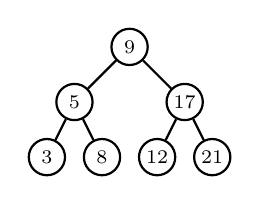
\begin{tikzpicture}[bt, level 1/.style={sibling distance=14mm}, level 2/.style={sibling distance=7mm}]
\node{9} child{node{5} child{node{3}} child{node{8}}} child{node{17} child{node{12}} child{node{21}}};
\end{tikzpicture}\\[-1pt]{\scriptsize tree S}
\end{minipage}

\Lcol[0.49]
\pt{(a) Pseudocode}
\begin{algo}{Algorithm 14a}{BST check with ranges}
\Require node; open range (low, high)
\Ensure true iff the subtree is a valid BST in range
\Init{\Call{IsBST}{root, $-\infty$, $+\infty$}}
\Procedure{IsBST}{node, low, high}
  \If{node $=$ NULL}
    \State \Return true
  \EndIf
  \If{node.data $\le$ low \textbf{or} node.data $\ge$ high}
    \State \Return false
  \EndIf
  \If{\Call{IsBST}{node.left, low, node.data} $=$ false}
    \State \Return false
  \EndIf
  \State \Return \Call{IsBST}{node.right, node.data, high}
\EndProcedure
\end{algo}
\Rcol[0.49]
\pt{(b) Worked example} {\footnotesize Tree P: 12 is the left child of 5 but not below 5.}\par
{\scriptsize
\begin{tabularx}{\linewidth}{@{}r l l l Y@{}}
\toprule
\# & Call & Range & Lines & Returns \\
\midrule
1 & 5 & $(-\infty,+\infty)$ & 2,5,8,9 & false \\
2 & 12 & $(-\infty,5)$ & 2,5,6 & \textbf{false} (12 out of range) \\
\bottomrule
\end{tabularx}}
{\footnotesize Tree S: every node is inside its range.}\par
{\scriptsize
\begin{tabularx}{\linewidth}{@{}r l l l Y@{}}
\toprule
\# & Call & Range & Lines & Returns \\
\midrule
1 & 9 & $(-\infty,+\infty)$ & 2,5,8,11 & true \\
2 & 5 & $(-\infty,9)$ & 2,5,8,11 & true \\
3 & 3 & $(-\infty,5)$ & 2,5,8,11 & true \\
4 & \nul{3.L} & $(-\infty,3)$ & 2,3 & true \\
5 & \nul{3.R} & $(3,5)$ & 2,3 & true \\
6 & 8 & $(5,9)$ & 2,5,8,11 & true \\
7 & \nul{8.L} & $(5,8)$ & 2,3 & true \\
8 & \nul{8.R} & $(8,9)$ & 2,3 & true \\
9 & 17 & $(9,+\infty)$ & 2,5,8,11 & true \\
10 & 12 & $(9,17)$ & 2,5,8,11 & true \\
11 & \nul{12.L} & $(9,12)$ & 2,3 & true \\
12 & \nul{12.R} & $(12,17)$ & 2,3 & true \\
13 & 21 & $(17,+\infty)$ & 2,5,8,11 & true \\
14 & \nul{21.L} & $(17,21)$ & 2,3 & true \\
15 & \nul{21.R} & $(21,+\infty)$ & 2,3 & true \\
\bottomrule
\end{tabularx}}
{\footnotesize ISBST(P) $=$ \textbf{false}, ISBST(S) $=$ \textbf{true} $=$ expected.}
\Ecol
\Lcol[0.49]
\pt{(c) Frequency count} {\footnotesize worst case $=$ valid BST.}\par
{\footnotesize\begin{tabularx}{\linewidth}{@{}c Y c c c c@{}}\toprule
Line & Operation & Cost & Freq. & S & P \\ \midrule
2 & test node $=$ NULL & 1 & $2n+1$ & 15 & 2 \\
3 & return true & 1 & $n+1$ & 8 & 0 \\
5 & test out of range & 1 & $n$ & 7 & 2 \\
6 & return false & 1 & 0 & 0 & 1 \\
8 & test left subtree & 1 & $n$ & 7 & 1 \\
9 & return false & 1 & 0 & 0 & 1 \\
11 & return right subtree & 1 & $n$ & 7 & 0 \\ \midrule
 & \textbf{Total} & & $\mathbf{6n+2}$ & \textbf{44} & \textbf{7} \\ \bottomrule
\end{tabularx}}
\Rcol[0.49]
\pt{(d) Final complexity.} \textbf{Worst} $\Theta(n)$ ($6n+2$, any valid BST). \textbf{Best} $\Theta(1)$: a violation at the root's left child is caught on call 2 (P: 7 lines). \textbf{Extra space} $\Theta(h)$.
\Ecol
\Lcol[0.47]
\begin{algo}{Algorithm 14b}{BST check with inorder}
\Require node; prev (by reference)
\Ensure true iff inorder is strictly increasing
\Init{prev $\gets -\infty$;\ \Call{IsBSTIn}{root, prev}}
\Procedure{IsBSTIn}{node, prev}
  \If{node $=$ NULL}
    \State \Return true
  \EndIf
  \If{\Call{IsBSTIn}{node.left, prev} $=$ false}
    \State \Return false
  \EndIf
  \If{node.data $\le$ prev}
    \State \Return false
  \EndIf
  \State prev $\gets$ node.data
  \State \Return \Call{IsBSTIn}{node.right, prev}
\EndProcedure
\end{algo}
\Rcol[0.51]
\pt{Twist: inorder solution.} A BST's inorder is strictly increasing, so compare each node with the previous value. On P the first comparison is only at the leftmost node 21; the next, $12\le21$, fails:\par
{\scriptsize
\begin{tabularx}{\linewidth}{@{}r l l l Y@{}}
\toprule
\# & Call & Lines & prev & Returns \\
\midrule
1 & 5 & 2,5,6 & --- & false \\
2 & 12 & 2,5,8,9 & 12 $\le$ 21 & \textbf{false} \\
3 & 21 & 2,5,8,11,12 & $-\infty$ $\to$ 21 & true \\
4 & \nul{21.L} & 2,3 & --- & true \\
5 & \nul{21.R} & 2,3 & --- & true \\
\bottomrule
\end{tabularx}}
{\footnotesize On S, prev runs $-\infty\to3\to5\to8\to9\to12\to17\to21$: true. Valid BST: line 2 $2n{+}1$, line 3 $n{+}1$, lines 5, 8, 11, 12 $n$ each, lines 6, 9 zero, so $T=7n+2$ (51 for S); 16 on P.}\par
\textbf{Comparison.} Worst case both $\Theta(n)$: $6n+2$ vs.\ $7n+2$ (inorder spends one more line per node on prev). Best cases differ: ranges can reject at the root's left child, $\Theta(1)$ (7 on P); inorder makes its first comparison only after reaching the leftmost node, so its earliest rejection costs $\Theta(d)$, $d$ = depth of the leftmost node (16 on P).
\Ecol

%==================================================================
\qhead{15}{8}{Vertical order traversal}
\noindent\begin{minipage}[c]{0.72\linewidth}
\pt{Idea.} Level order on (node, distance) pairs; append each value to its column's list. Level order is top to bottom, left to right, so each column is already in the required order. Track minD and maxD; every column between them is non-empty (distance changes by 1 per edge).
\end{minipage}\hfill
\begin{minipage}[c]{0.26\linewidth}\centering
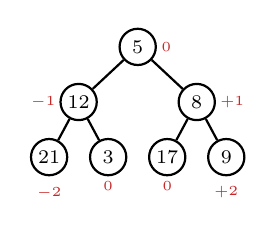
\begin{tikzpicture}[bt, level 1/.style={sibling distance=15mm}, level 2/.style={sibling distance=7.5mm}]
\node[label={[dl]right:0}]{5}
  child{node[label={[dl]left:$-1$}]{12} child{node[label={[dl]below:$-2$}]{21}} child{node[label={[dl]below:0}]{3}}}
  child{node[label={[dl]right:$+1$}]{8} child{node[label={[dl]below:0}]{17}} child{node[label={[dl]below:$+2$}]{9}}};
\end{tikzpicture}
\end{minipage}

\Lcol[0.47]
\pt{(a) Pseudocode}
\begin{algo}{Algorithm 15}{Vertical order traversal}
\Require pointer root to the root
\Ensure columns from leftmost to rightmost distance
\Init{\Call{Vertical}{root}}
\Procedure{Vertical}{root}
  \If{root $=$ NULL}
    \State \Return
  \EndIf
  \State cols $\gets$ empty map distance $\to$ list
  \State minD $\gets 0$;\ maxD $\gets 0$
  \State Q $\gets$ empty queue \Comment{(node, d) pairs}
  \State \Call{Enqueue}{Q, (root, 0)}
  \While{Q is not empty}
    \State (node, d) $\gets$ \Call{Dequeue}{Q}
    \State \Call{Append}{cols[d], node.data}
    \If{d $<$ minD}
      \State minD $\gets$ d
    \EndIf
    \If{d $>$ maxD}
      \State maxD $\gets$ d
    \EndIf
    \If{node.left $\neq$ NULL}
      \State \Call{Enqueue}{Q, (node.left, d$-1$)}
    \EndIf
    \If{node.right $\neq$ NULL}
      \State \Call{Enqueue}{Q, (node.right, d$+1$)}
    \EndIf
  \EndWhile
  \For{d $\gets$ minD \textbf{to} maxD}
    \For{$j \gets 0$ \textbf{to} \Call{Size}{cols[d]} $-1$}
      \State \textbf{print} cols[d][$j$]
    \EndFor
  \EndFor
\EndProcedure
\end{algo}
\Rcol[0.51]
\pt{(b) Worked example} {\footnotesize One row per pass; $v_d$ $=$ value $v$ at distance $d$.}\par
{\scriptsize
\begin{tabularx}{\linewidth}{@{}r Y l l l Y@{}}
\toprule
Pass & Queue before & Deq. & cols[d] (line 11) & 13/16 & Queue after \\
\midrule
1 & 5$_{0}$ & 5$_{0}$ & [0]$=$[5] & --- & 12$_{-1}$ 8$_{+1}$ \\
2 & 12$_{-1}$ 8$_{+1}$ & 12$_{-1}$ & [$-$1]$=$[12] & min$\gets$$-1$ & 8$_{+1}$ 21$_{-2}$ 3$_{0}$ \\
3 & 8$_{+1}$ 21$_{-2}$ 3$_{0}$ & 8$_{+1}$ & [+1]$=$[8] & max$\gets$$+1$ & 21$_{-2}$ 3$_{0}$ 17$_{0}$ 9$_{+2}$ \\
4 & 21$_{-2}$ 3$_{0}$ 17$_{0}$ 9$_{+2}$ & 21$_{-2}$ & [$-$2]$=$[21] & min$\gets$$-2$ & 3$_{0}$ 17$_{0}$ 9$_{+2}$ \\
5 & 3$_{0}$ 17$_{0}$ 9$_{+2}$ & 3$_{0}$ & [0]$=$[5, 3] & --- & 17$_{0}$ 9$_{+2}$ \\
6 & 17$_{0}$ 9$_{+2}$ & 17$_{0}$ & [0]$=$[5, 3, 17] & --- & 9$_{+2}$ \\
7 & 9$_{+2}$ & 9$_{+2}$ & [+2]$=$[9] & max$\gets$$+2$ & empty \\
\bottomrule
\end{tabularx}}
{\footnotesize Lines 25--29 then print d $=-2..+2$: \textbf{$-2$: 21 $\mid$ $-1$: 12 $\mid$ 0: 5, 3, 17 $\mid$ $+1$: 8 $\mid$ $+2$: 9} $=$ expected (3 before 17 by level order).}\par\vspace{3pt}
\pt{(c) Frequency count} {\footnotesize $c=$ maxD $-$ minD $+1$ columns ($c=5$); $a$, $b$ updates on lines 13, 16 ($2, 2$). A new minimum is always one below the old (its parent was already seen), likewise the maximum, so $a+b=c-1$.}\par
{\footnotesize\begin{tabularx}{\linewidth}{@{}c Y c c c@{}}\toprule\fhead
2 & test root & 1 & 1 & 1 \\
5 & cols $\gets$ empty & 1 & 1 & 1 \\
6 & minD, maxD $\gets 0$ & 1 & 1 & 1 \\
7 & Q $\gets$ empty & 1 & 1 & 1 \\
8 & Enqueue(root, 0) & 1 & 1 & 1 \\
9 & test Q not empty & 1 & $n+1$ & 8 \\
10 & Dequeue & 1 & $n$ & 7 \\
11 & Append to cols[d] & 1 & $n$ & 7 \\
12 & test d $<$ minD & 1 & $n$ & 7 \\
13 & minD $\gets$ d & 1 & $a$ & 2 \\
15 & test d $>$ maxD & 1 & $n$ & 7 \\
16 & maxD $\gets$ d & 1 & $b$ & 2 \\
18 & test left & 1 & $n$ & 7 \\
19 & Enqueue left & 1 & $n_L$ & 3 \\
21 & test right & 1 & $n$ & 7 \\
22 & Enqueue right & 1 & $n_R$ & 3 \\
25 & for d: init / test / incr. & 1 & $1$ / $c{+}1$ / $c$ & 1/6/5 \\
26 & for $j$: init / test / incr. & 1 & $c$ / $n{+}c$ / $n$ & 5/12/7 \\
27 & print & 1 & $n$ & 7 \\ \midrule
 & \textbf{Total} & & $\mathbf{11n{+}4c{+}a{+}b{+}7}$ & \textbf{108} \\ \bottomrule
\end{tabularx}}
{\footnotesize With $n_L{+}n_R=n{-}1$, $a{+}b=c{-}1$: $T=11n+5c+6$; check $77+25+6=108$.~\checkmark}
\Ecol
\pt{(d) Final complexity.} $2\le c\le n$ (for $n\ge2$), so $11n+16\le T(n)\le16n+6$: \textbf{best} $=$ \textbf{worst} $=\Theta(n)$. Worst count: a one-sided chain ($c=n$); best: a zigzag chain ($c=2$). Grouping costs one line per node (hash map, or an array of $2n-1$ lists indexed by $d+n-1$); printing costs $3n+4c+2$. \textbf{Extra space} $\Theta(n)$ (columns hold all values; queue up to $w$ pairs).
\pt{Twist (number of columns).} Each column holds at least one node, so $c\le n$, reached by a chain that always goes the same way (distances $0,-1,\dots,-(n-1)$). Distances can range over $2n-1$ values, $-(n-1)..n-1$, but at most $n$ are occupied. A single node has 1 column, a zigzag chain only 2, and a complete tree of height $h$ has $2h+1$ (5 here).

\end{document}
